Dopo aver analizzato gli strumenti che già hanno provato a sviluppare un covert channel tramite ICMP e 
dopo aver analizzato metodologie sfruttabili per poter nascondere i dati; 
procediamo nel svilupparne uno; il cui codice è contenuto in una repository GitHub \cite{repoGITHUB}.  
\vspace{2ex} \newline 
Per la definizione della struttura, si è preso spunto da 
\textbf{icmp tunnel} \cite{icmp-tunnel}; il cui schema generale di funzionamento 
viene mostrato nella Figura \ref{fig:icmpTunnel:architettura:generale}.
\vspace{3ex}\newline
\begin{center} 
    \captionof{figure}{Architettura generale di \textbf{icmp tunnel} \cite{icmp-tunnel}}
    \label{fig:icmpTunnel:architettura:generale} 
    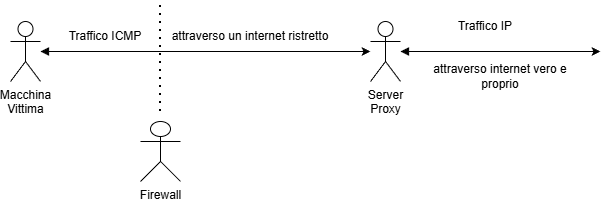
\includegraphics[width=0.7\textwidth]{../img/ICMPtunnel/architettura_generale.png} 
\end{center} 
La Figura \ref{fig:icmpTunnel:architettura:vittima} mostra la struttura della comunicazione fra la macchina vittima e il proxy.
\textit{Icmp tunnel} che è in esecuzione sulla macchina vititma, reindirizza il traffico IP ad un interfaccia virtuale per poi reinoltrarlo 
al proxy tramite il protocollo ICMP. 
\vspace{3ex}\newline
\begin{center} 
    \captionof{figure}{Comunicazione vitttima-proxy in \textbf{icmp tunnel} \cite{icmp-tunnel}}
    \label{fig:icmpTunnel:architettura:vittima} 
    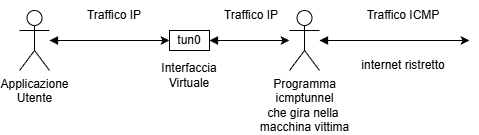
\includegraphics[width=0.65\textwidth]{../img/ICMPtunnel/architettura_vittima.png} 
\end{center} 
Il proxy intanto rimane in ascolto di questi pacchetti ICMP e poi li invia, utilizzando il protocollo IP, verso la destinazione finale. 
Successivamente i pacchetti in entrata nel proxy, che contengono le informazioni da inoltrare alla macchina vittima, 
vengono incapsulati tramite il protocollo ICMP ed inoltrati alla vittima.  
La Figura \ref{fig:icmpTunnel:architettura:proxy} mostra la struttura di quest'ultima parte. 
\vspace{3ex}\newline
\begin{center} 
    \captionof{figure}{Comunicazione proxy-internet in \textbf{icmp tunnel} \cite{icmp-tunnel}}
    \label{fig:icmpTunnel:architettura:proxy} 
    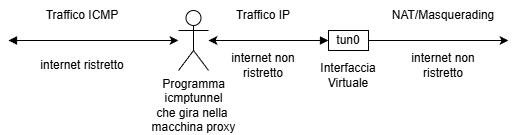
\includegraphics[width=0.65\textwidth]{../img/ICMPtunnel/architettura_proxy.png} 
\end{center} 
\vspace{2ex} 
Alcuni aspetti da considerare, utili l'implementazione della comunicazione, sono: 
\begin{enumerate}
    \item La \textbf{presenza di più proxy intermediari} fra l'attaccante e la vittima.  
    Sebbene sia possibile usare un singolo proxy, l'utilizzo di più macchine 
    proxy permette di nascondere meglio la comunicazione. 
    \vspace{1ex} \newline
    Con un solo proxy, il sistema di difesa potrebbe notare che tutto 
    il traffico ICMP viene inviato ad un'unica sorgente. 
    Se invece si utilizzano più proxy, il traffico può essere distribuito fra più destinatari diversi. 
    \item La \textbf{quantità di dati} che si vuole inviare. 
    Se mai si volesse esfiltrare un file; la grande quantità di dati potrebbe generare rumore. 
    \vspace{1ex} \newline 
    Si deve tenere conto di un \textbf{limite massimo} di dati inviabili in un intervallo di tempo ed 
    un \textbf{periodo di riposo} che deve trascorrere prima di poterne inviare altri.
    \item La \textbf{trasmissione dei dati in chiaro} permettera a chiunque di leggerne il contenuto. 
    Un sistema di difesa che fà uso dell'ispezione approfondita dei pacchetti (Deep Packet Inspection) potrebbe rilevare la comunicazione. 
    Tuttavia anche la \textbf{trasmissione di dati cifrati} potrebbe destare sospetti. 
    \vspace{1ex} \newline 
    Si devono quindi poter mandare dati in maniera cifrata ma che al tempo stesso non sembrino cifrati.  
    Al momento non si è trovato un metodo efficace a parte l'inserimento di dati in forma numerica 
    (anche se non viene considerata una cifratura ma pià una decodifica del carattere\footnote{Questo perchè un carattere ASCII può essere codificato tramite un numero intero.}). 
    \item I \textbf{messaggi di tipo Request}, inviano un messaggio di richiesta e poi aspettano una risposta 
    avente gli stessi dati ricevuti. 
    Si avranno quindi due messaggi identici (tranne per il campo che indica il tipo di messaggio). 
    Ciò risulta un problema se la dimensione del campo contenente i dati è eccessiva. 
    Inoltre il numero di messaggi inviati raddoppierà.    
    \vspace{1ex} \newline 
    Delle possibili soluzioni sono: 
    \begin{itemize} 
        \item l'uso dei solo messaggi messaggi di risposta (di tipo \textbf{Reply}). 
        Tuttavia sarà anomalo che il numero delle risposte non combaci con 
        quello delle richieste. 
        \item la disabilitazione, se possibile, dell'invio da parte del sistema delle risposte 
        così da mandare una risposta specifica (che non ripeterà il contenuto della richiesta). 
        In questo caso ad una richiesta combacierà una risposta sebbene 
        non conforme agli standard. 
    \end{itemize} 
\end{enumerate} 

